\documentclass[a4paper,12pt]{article}

\usepackage{graphicx}	% Pour importer des images
\usepackage[left=2.5cm,right=2.5cm,top=2cm,bottom=3.5cm]{geometry} %Configuration de la page
\usepackage{amsmath}
\usepackage{amsthm}
\usepackage{hyperref}
\usepackage{float}
\usepackage{booktabs}
\usepackage[T1]{fontenc}
\usepackage[table]{xcolor}
\usepackage{tikz}
\usepackage{pgfplots}
\pgfplotsset{compat=1.18}

\newtheorem*{remark}{Remark}


\begin{document}

\title{Note on Hypotension Prediction}

\author{Bob Aubouin--Pairault}
\maketitle


\section{Goal of the document}

The goal of this document is to summarize all the work done on the hypotension prediction.


\section{Abstract sent to the conference}

Intraoperative hypotension (IOH) is common during surgical procedures. It may be caused by anesthesia drugs, underlying  comorbidities of the patient such as heart failure, or by the surgical procedure. There are strong associations between IOH and postoperative organ complications, thus the ability to predict IOH to support the clinician is an attractive prospect. In this presentation, the prediction of hypotension during general anesthesia using physiological signal is investigated. \medskip

Recently, some research has been focused on trying to predict hypotension events occurring during surgeries using machine learning techniques \cite{hatibMachinelearningAlgorithmPredict2018}. However, this methodology has been subject to some questioning \cite{enevoldsenPerformanceHypotensionPrediction2022}, \cite{smithConHypotensionPrediction2023}. Especially, the database seems to be biased, and the evaluations are not compared to a relevant baseline. A new methodology addressing the arisen questions is proposed here. Exploratory investigations are illustrated using the open source VitalDB database \cite{leeVitalDBHighfidelityMultiparameter2022} and standard machine learning algorithms. In addition, the explainability of the prediction is studied to provide more information to the anesthesiologist.


\section{Feature selection}


\begin{table}
\small
\begin{center}
\center
\rowcolors{2}{white}{gray!20}
\begin{tabular}{p{0.17\textwidth}|p{0.4\textwidth}|c|c}
\textbf{Feature} & \textbf{Description} & \textbf{VitalDB Name} & \textbf{Code name} \\
\midrule
Mean Arterial Pressure & Average blood pressure during a cardiac cycle & Solar8000/ART\_MBP & mbp\\
Systolic Blood Pressure & Maximum blood pressure during a cardiac cycle & Solar8000/ART\_SBP & sbp \\
Diastolic Blood Pressure & Minimum blood pressure during a cardiac cycle & Solar8000/ART\_DBP & dbp \\
Heart Rate & Number of heart beats per minute & Solar8000/HR & hr\\
Respiration Rate & Number of breaths per minute & Solar8000/RR & rr\\
Oxygen Saturation & Percentage of hemoglobin saturated with oxygen & Solar8000/PLETH\_SPO2 & spo2 \\
End Tidal CO2 & Concentration of carbon dioxide at the end of an exhaled breath & Solar8000/ETCO2 & etco2 \\
Propofol target & Target of propofol concentration in the blood & Orchestra/PPF20\_CT & pp\_ct\\
 MAC & minimum alveolar concentration (MAC), for volatile anesthetics &  Primus/MAC & mac\\
 BIS & Bispectral index (depth of hypnosis) & BIS/BIS & bis
\end{tabular}
\caption{List of the dynamic features that can be linked to the prediction of hypotension.}
\end{center}
\end{table}

\begin{table}
\begin{center}
\rowcolors{2}{white}{gray!20}
\begin{tabular}{c|p{0.4\textwidth}|c}
\textbf{Feature} & \textbf{Description} & \textbf{VitalDB Name} \\
\midrule
Age & Age & age \\
BMI & Body mass index & bmi \\
ASA & Physical statut classification & asa \\
Creatinine & Preoperative creatinine concentration in the blood & preop\_cr \\
Hypertension & Preoperative hypertension of the patient & preop\_htn \\
operation name & operation name (if we can proceed text) & opname
\end{tabular}
\caption{List of the static features that can be linked to the prediction of hypotension.}
\end{center}
\end{table}

\section{Patient selection}
Patients are selected using the following criteria:

\begin{itemize}
    \item The patient is under general anesthesia
    \item The patient is not in emergency
    \item Arterial blood pressure is invasively measured
    \item The patient is major (age > 18yr)
    \item The operation is not a transplantation (no "transplant" in operation name
    \item The anesthesia duration is at least one hour.
    \item More than 70\% of the previously listed signals are available (no Nan) 
    \item All the static information about the patient are available
\end{itemize}

\section{Hypotension labelling}


For this first work, we will use the standard labelling of hypotension event used in the literature. A hypotension event is defined as a mean arterial pressure (MAP) lower than 65mmHg for more than 1 minute. \medskip

\textbf{Idea For future work:}



As there is no clearly adopted definition of hypotension event automatic labelling of the data could be an arduous task. In the literature, it exists two different quantitative ways to define hypotension: using a relative threshold from baseline of mean or systolic blood pressure or using an absolute threshold on those values. Because the true blood pressure baseline might be hard to obtain, the first method is often inapplicable in practice. The second method, easier to implement is actually used for most of the research papers on this topic. However, this labelling method lacks of patient specificity, in fact, the baseline MAP of some patient might be close to the threshold such that labelled situation could correspond to normal situation. \medskip

For our approach, a new method for labelling the hypotension events is proposed. Our guess is that the anesthesiologists in the surgery room are the more appropriate to diagnostic IOH. Thus, the idea is to take advantage of our future point of view to assesse the potential of a low blood pressure to correspond to an IOH thanks to the anesthesiologist reaction in the minutes following the event. \medskip

To treat an IOH event different possibilities can be used depending on the cause:
\begin{itemize}
    \item If the IOH is due to a too deep hypnosis, the hypnotic drug dosage must be adjusted.
    \item If the IOH is due to a too important fluid loss, the missing fluid must be replaced with blood or cristalloid.
    \item If the cause is the vasodilatation of the vessels, vasopressor drugs must be injected.
\end{itemize}

The first possibility can be verified easily using data from hypnotic drug dosage (i.e. propofol, desflurane or sevoflurane). The second also correspond to changes in drug injection profiles. However, of those drugs are mostly injected by bolus and only the total amount of drug injected during the anesthesia is recorded in vitalDB. The same problem applied to fluid replacement where only the total amount of fluid lost and injected is available in vitalDB. \medskip

One idea to label the data could be to ask the anesthesiologist to label a part of the data. The train a model to predict the label of the anesthesiologist thanks to past and future data around the event (in contrast to the final model which will only used past data). This model could then be used to label the rest of the data. \medskip


\section{Framing the problem}

Framing the problem is an important step in the machine learning process for clinical application. In fact recent paper \cite{lauritsenFramingMachineLearning2021} have shown that the way the problem is framed can have a huge impact on the performance of the model and the way it could be used in practice. \medskip

In the litterature, \cite{hatibMachinelearningAlgorithmPredict2018} and \cite{leeDeepLearningModels2021} have used a "fixed time to onset" approach. For this approach, the model is trained to respond to one particular question: "Will the patient have a hypotension event in the next $X$ minutes?" where $X$ was 5, 10 or 15 minutes. If this type of framing leads to the best algorithmic performances, this does not respond to a solid clinical question. In fact, with this approach a perfect model would be useless in practice. A more relevant framing have been proposed in \cite{enevoldsenSelectionBiasHypotension2023} where the question is: "Will the patient have a hypotension event in the next $3$ to $10$ minutes?". This framing correspond to a sliding window approach. An illustration of the existing approach and the one proposed here is given in Fig.~\ref{fig:framing}.

\begin{figure}[h]
    \centering
    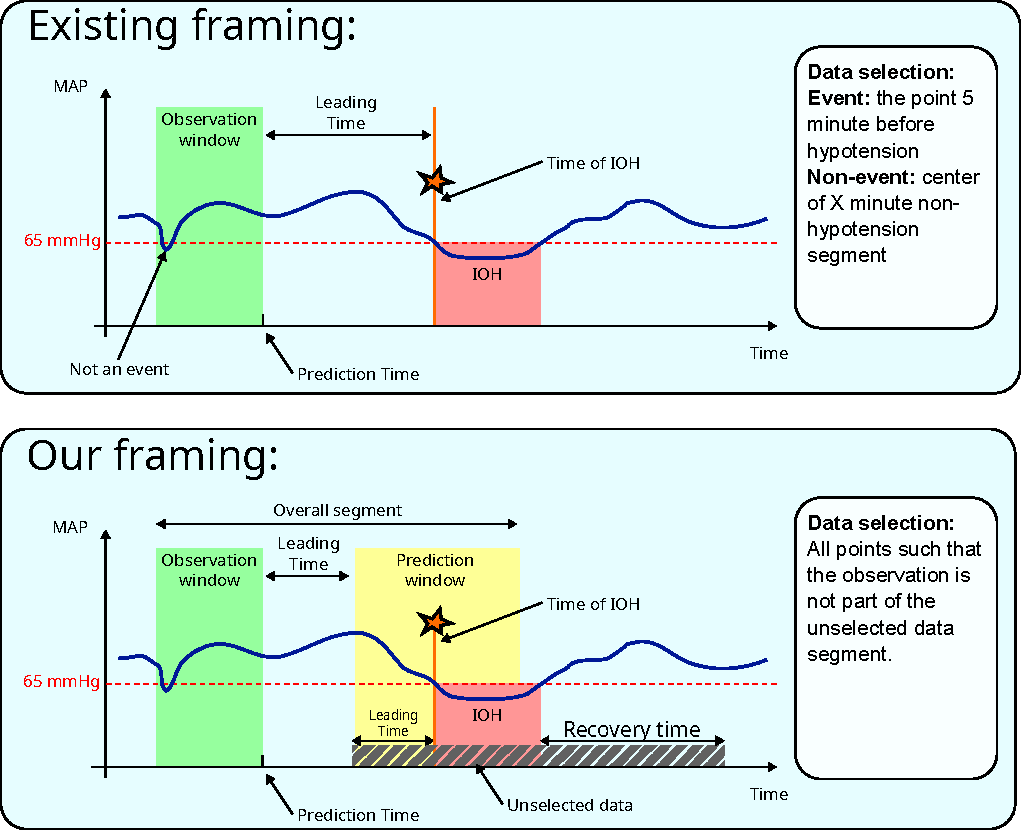
\includegraphics[width=\textwidth]{figures/framing.pdf}
    \caption{Illustration of the different framing of the problem.}
    \label{fig:framing}
\end{figure}

The parameters of our framing are the following:
\begin{itemize}
    \item The size of the observation window (first try with 3 minutes)
    \item The leading time (first try with 3 minutes)
    \item The size of the prediction window (first try with 7 minutes)
    \item The recovery time (first try with 15 minutes, should not change too much)
\end{itemize}

The impact of those parameters must be studied in this work or the followings.

\section{Data pre-processing}

The following flow chart describes the data selection of each segment of the data. 

\begin{figure}[h]
    \centering
    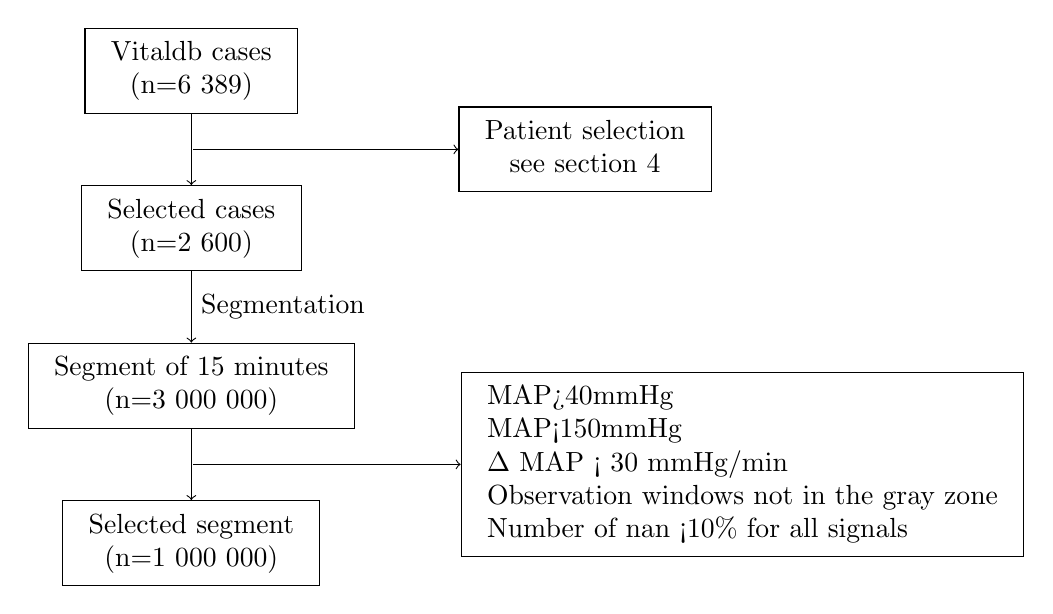
\begin{tikzpicture}
    \node (vdb) at (0, 0) [draw, rectangle, minimum width=2cm, minimum height=1cm] {\begin{tabular}{c} Vitaldb cases \\ (n=6 389) \end{tabular}};

    \node (cases) [draw, rectangle, below of=vdb, yshift= -1cm, minimum width=2cm, minimum height=1cm] {\begin{tabular}{c} Selected cases \\ (n=2 600) \end{tabular}};

    \node (features) [draw, rectangle, below of=cases, yshift= -1cm, minimum width=2cm, minimum height=1cm] {\begin{tabular}{c} Segment of 15 minutes \\ (n=3 000 000) \end{tabular}};

    \node (selected_features) [draw, rectangle, below of=features, yshift= -1cm, minimum width=2cm, minimum height=1cm] {\begin{tabular}{c} Selected segment \\ (n=1 000 000) \end{tabular}};

    \draw [->] (vdb) -- (cases) node (arrow1) [midway, xshift=-1mm] {};
    \draw [->] (cases) -- (features)node [midway, right] {Segmentation};
    \draw [->] (features) -- (selected_features) node (arrow3) [midway, xshift=-1mm] {};


    \node (patient_select) [draw, rectangle, right of=vdb, xshift= 4cm, yshift=-1cm, minimum width=2cm, minimum height=1cm] {\begin{tabular}{c} Patient selection \\ see section 4 \end{tabular}};
    \draw [<-] (patient_select) -- (arrow1);

    \node (feature_select) [draw, rectangle, right of=features, xshift= 6cm, yshift= -1cm, minimum width=2cm, minimum height=1cm] {\begin{tabular}{l} MAP>40mmHg \\ MAP<150mmHg \\ $\Delta$ MAP < 30 mmHg/min \\ Observation windows not in the gray zone \\ Number of nan <10\% for all signals \end{tabular}};
    \draw [<-] (feature_select) -- (arrow3);
\end{tikzpicture}
    \caption{Data pre-processing flow chart}
    \label{fig:preprocessing}
\end{figure}



\section{Evaluation}

To fairly evaluate the potential of our method against baseline and evaluate uncertainty on our results a Leave One Out Cross-Validation (LOOCV) is used \cite{meghnoudjSparseOptimalControlbased2024}. This method consist on partitioning the set of patient in $k$ distinct subset. Then to loops are nested, in the outer one a subset is leaved out before any training on the data and is used as a test set to assesse the performance of the method. In the inner one, a subset is leaved out to be used as a validation set for the hyperparameters tuning. This method is illustrated on Fig.~\ref{fig:loocv}.

\begin{figure}
    \centering
    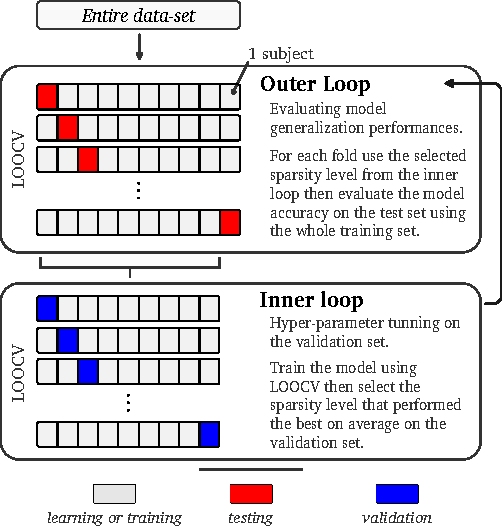
\includegraphics[width=0.7\textwidth]{figures/chap_1_NLOO.pdf}
    \caption{Illustration of Leave one out cross validation (from \cite{meghnoudjSparseOptimalControlbased2024})}
    \label{fig:loocv}
\end{figure}

In this work the metric used is the Aera Under the Receiver operating characteristic curve (AUC) \cite{masonAreasRelativeOperating2002a}. This curve evaluates the ability of a binary classifier at different threshold value and is usually used in medical field. It is the plot of the True Positive error against the False positive error (or sensitivity against 1 - specificity). The way to associate a $p$-value to this metric must be inestigated in \cite{masonAreasRelativeOperating2002a}.

\section{Baseline}

A fair baseline for the prediction of hypotension have been recently published in \cite{jacquet-lagrezePredictionIntraoperativeHypotension2022}. In this article they demonstrate that both linear extrapolation of MAP value and last value of MAP are good baseline for the prediction of hypotension. In this work, we used the last value of MAP as a baseline, as it is simplest to implement. \medskip

Results of the baseline are given in Fig.~\ref{fig:baseline}.

\begin{figure}[h]
    \centering
    % This file was created with tikzplotlib v0.10.1.
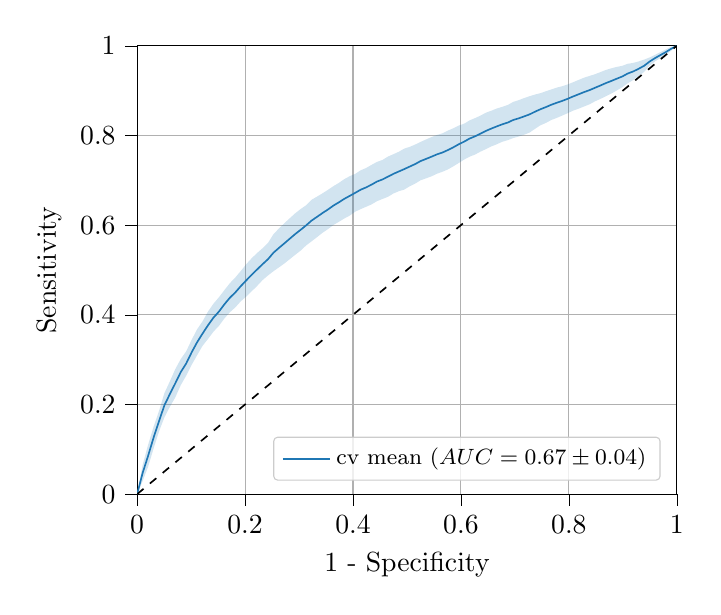
\begin{tikzpicture}

\definecolor{darkgray176}{RGB}{176,176,176}
\definecolor{lightgray204}{RGB}{204,204,204}
\definecolor{steelblue31119180}{RGB}{31,119,180}

\begin{axis}[
legend cell align={left},
legend style={
  fill opacity=0.8,
  draw opacity=1,
  text opacity=1,
  at={(0.97,0.03)},
  anchor=south east,
  draw=lightgray204
},
legend style={rounded corners=0.5mm, font=\footnotesize},
tick align=outside,
tick pos=left,
x grid style={darkgray176},
xlabel={1 - Specificity},
xmajorgrids,
xmin=0, xmax=1,
xtick style={color=black},
y grid style={darkgray176},
ylabel={Sensitivity},
ymajorgrids,
ymin=0, ymax=1,
ytick style={color=black}
]
\path [fill=steelblue31119180, fill opacity=0.2]
(axis cs:0,0)
--(axis cs:0,0)
--(axis cs:0.0101010101010101,0.0290349297878335)
--(axis cs:0.0202020202020202,0.060454429920711)
--(axis cs:0.0303030303030303,0.101047584275281)
--(axis cs:0.0404040404040404,0.139351034140325)
--(axis cs:0.0505050505050505,0.171098234088693)
--(axis cs:0.0606060606060606,0.194715565175068)
--(axis cs:0.0707070707070707,0.215730718278744)
--(axis cs:0.0808080808080808,0.243089980699637)
--(axis cs:0.0909090909090909,0.264245458662335)
--(axis cs:0.101010101010101,0.288421073613483)
--(axis cs:0.111111111111111,0.309778066762688)
--(axis cs:0.121212121212121,0.330803341828769)
--(axis cs:0.131313131313131,0.346095664543095)
--(axis cs:0.141414141414141,0.362432696656044)
--(axis cs:0.151515151515152,0.375225148892526)
--(axis cs:0.161616161616162,0.391716483586593)
--(axis cs:0.171717171717172,0.405515597817263)
--(axis cs:0.181818181818182,0.416430306652205)
--(axis cs:0.191919191919192,0.429880904530132)
--(axis cs:0.202020202020202,0.440523418259981)
--(axis cs:0.212121212121212,0.452287091308384)
--(axis cs:0.222222222222222,0.464288662270891)
--(axis cs:0.232323232323232,0.477288055977727)
--(axis cs:0.242424242424242,0.487673147952431)
--(axis cs:0.252525252525253,0.497150515743615)
--(axis cs:0.262626262626263,0.50564881848661)
--(axis cs:0.272727272727273,0.514352089864354)
--(axis cs:0.282828282828283,0.524136658084681)
--(axis cs:0.292929292929293,0.533822720183591)
--(axis cs:0.303030303030303,0.543245960600113)
--(axis cs:0.313131313131313,0.554676441765618)
--(axis cs:0.323232323232323,0.56383649347456)
--(axis cs:0.333333333333333,0.57324834889736)
--(axis cs:0.343434343434343,0.582919526435142)
--(axis cs:0.353535353535354,0.591098713689954)
--(axis cs:0.363636363636364,0.600191802560265)
--(axis cs:0.373737373737374,0.607390390470973)
--(axis cs:0.383838383838384,0.614755228046438)
--(axis cs:0.393939393939394,0.621282488275542)
--(axis cs:0.404040404040404,0.629875764270055)
--(axis cs:0.414141414141414,0.635727377692046)
--(axis cs:0.424242424242424,0.640899918638662)
--(axis cs:0.434343434343434,0.646207200557807)
--(axis cs:0.444444444444444,0.65345976490859)
--(axis cs:0.454545454545455,0.658364373627733)
--(axis cs:0.464646464646465,0.663132846806713)
--(axis cs:0.474747474747475,0.670476968262848)
--(axis cs:0.484848484848485,0.675712091396864)
--(axis cs:0.494949494949495,0.679239482668169)
--(axis cs:0.505050505050505,0.686669455741936)
--(axis cs:0.515151515151515,0.692630652098976)
--(axis cs:0.525252525252525,0.70003597726398)
--(axis cs:0.535353535353535,0.704314637313909)
--(axis cs:0.545454545454546,0.708829657453376)
--(axis cs:0.555555555555556,0.714639115452409)
--(axis cs:0.565656565656566,0.71899833029763)
--(axis cs:0.575757575757576,0.724164507138654)
--(axis cs:0.585858585858586,0.731125861385702)
--(axis cs:0.595959595959596,0.73863330461267)
--(axis cs:0.606060606060606,0.746280804056094)
--(axis cs:0.616161616161616,0.752701596408378)
--(axis cs:0.626262626262626,0.757513135530153)
--(axis cs:0.636363636363636,0.764065477064363)
--(axis cs:0.646464646464647,0.769679082252671)
--(axis cs:0.656565656565657,0.775724767575321)
--(axis cs:0.666666666666667,0.78049044476985)
--(axis cs:0.676767676767677,0.786009752626088)
--(axis cs:0.686868686868687,0.789599653922063)
--(axis cs:0.696969696969697,0.794269868927868)
--(axis cs:0.707070707070707,0.797659669883366)
--(axis cs:0.717171717171717,0.801689509034105)
--(axis cs:0.727272727272727,0.806559904288977)
--(axis cs:0.737373737373737,0.814875402371818)
--(axis cs:0.747474747474748,0.822813881582026)
--(axis cs:0.757575757575758,0.828030378270688)
--(axis cs:0.767676767676768,0.834613625246324)
--(axis cs:0.777777777777778,0.839251538785974)
--(axis cs:0.787878787878788,0.844494592643222)
--(axis cs:0.797979797979798,0.849834052028163)
--(axis cs:0.808080808080808,0.855462287603708)
--(axis cs:0.818181818181818,0.859806227774874)
--(axis cs:0.828282828282828,0.864696076587655)
--(axis cs:0.838383838383838,0.869563407407876)
--(axis cs:0.848484848484849,0.876181261869315)
--(axis cs:0.858585858585859,0.881640980801661)
--(axis cs:0.868686868686869,0.887568685132135)
--(axis cs:0.878787878787879,0.893496029582882)
--(axis cs:0.888888888888889,0.900442015337844)
--(axis cs:0.898989898989899,0.907759256403589)
--(axis cs:0.909090909090909,0.916492236135167)
--(axis cs:0.919191919191919,0.923645924430268)
--(axis cs:0.929292929292929,0.932390995681463)
--(axis cs:0.939393939393939,0.941639612606365)
--(axis cs:0.94949494949495,0.955530536385906)
--(axis cs:0.95959595959596,0.965279624689285)
--(axis cs:0.96969696969697,0.972742625244099)
--(axis cs:0.97979797979798,0.980153918771255)
--(axis cs:0.98989898989899,0.989414164848848)
--(axis cs:1,1)
--(axis cs:1,1)
--(axis cs:1,1)
--(axis cs:0.98989898989899,0.99789353693612)
--(axis cs:0.97979797979798,0.991986911285862)
--(axis cs:0.96969696969697,0.986008514400581)
--(axis cs:0.95959595959596,0.979750269262035)
--(axis cs:0.94949494949495,0.973985635240625)
--(axis cs:0.939393939393939,0.969195883051465)
--(axis cs:0.929292929292929,0.965177857421406)
--(axis cs:0.919191919191919,0.961874053087932)
--(axis cs:0.909090909090909,0.95988857618616)
--(axis cs:0.898989898989899,0.955367717397884)
--(axis cs:0.888888888888889,0.952951911505238)
--(axis cs:0.878787878787879,0.94985929835559)
--(axis cs:0.868686868686869,0.946194805117624)
--(axis cs:0.858585858585859,0.941420982861642)
--(axis cs:0.848484848484849,0.936611880056885)
--(axis cs:0.838383838383838,0.932823622776364)
--(axis cs:0.828282828282828,0.928942793475934)
--(axis cs:0.818181818181818,0.923968666901542)
--(axis cs:0.808080808080808,0.918812091451753)
--(axis cs:0.797979797979798,0.913956730902923)
--(axis cs:0.787878787878788,0.909916743242928)
--(axis cs:0.777777777777778,0.906843337629898)
--(axis cs:0.767676767676768,0.902695327158153)
--(axis cs:0.757575757575758,0.898719381635834)
--(axis cs:0.747474747474748,0.894332608864433)
--(axis cs:0.737373737373737,0.891327802582523)
--(axis cs:0.727272727272727,0.887598781159647)
--(axis cs:0.717171717171717,0.883487943787248)
--(axis cs:0.707070707070707,0.878767415713378)
--(axis cs:0.696969696969697,0.874907452145613)
--(axis cs:0.686868686868687,0.868151385937552)
--(axis cs:0.676767676767677,0.86391648377241)
--(axis cs:0.666666666666667,0.860272475304706)
--(axis cs:0.656565656565657,0.855286376847829)
--(axis cs:0.646464646464647,0.850963408253341)
--(axis cs:0.636363636363636,0.844428364244703)
--(axis cs:0.626262626262626,0.838806871804665)
--(axis cs:0.616161616161616,0.833739847693108)
--(axis cs:0.606060606060606,0.826378336697688)
--(axis cs:0.595959595959596,0.822070043419961)
--(axis cs:0.585858585858586,0.816054050344421)
--(axis cs:0.575757575757576,0.810809496281122)
--(axis cs:0.565656565656566,0.804755704818173)
--(axis cs:0.555555555555556,0.801115988419499)
--(axis cs:0.545454545454546,0.796506686813776)
--(axis cs:0.535353535353535,0.791120264247179)
--(axis cs:0.525252525252525,0.785722643917833)
--(axis cs:0.515151515151515,0.779749726371784)
--(axis cs:0.505050505050505,0.774571298310221)
--(axis cs:0.494949494949495,0.7706841607094)
--(axis cs:0.484848484848485,0.76362693670135)
--(axis cs:0.474747474747475,0.758188835155695)
--(axis cs:0.464646464646465,0.752826523452072)
--(axis cs:0.454545454545455,0.74538136392171)
--(axis cs:0.444444444444444,0.741004003836482)
--(axis cs:0.434343434343434,0.734415414781202)
--(axis cs:0.424242424242424,0.72739340481984)
--(axis cs:0.414141414141414,0.722280143102898)
--(axis cs:0.404040404040404,0.714153388299289)
--(axis cs:0.393939393939394,0.709229837400291)
--(axis cs:0.383838383838384,0.70257111515409)
--(axis cs:0.373737373737374,0.69419988504724)
--(axis cs:0.363636363636364,0.686915885697048)
--(axis cs:0.353535353535354,0.678658040487084)
--(axis cs:0.343434343434343,0.670944815338597)
--(axis cs:0.333333333333333,0.663665705731419)
--(axis cs:0.323232323232323,0.656538993495923)
--(axis cs:0.313131313131313,0.644255084900095)
--(axis cs:0.303030303030303,0.635999315064382)
--(axis cs:0.292929292929293,0.626406920462803)
--(axis cs:0.282828282828283,0.615387849672957)
--(axis cs:0.272727272727273,0.604223263432018)
--(axis cs:0.262626262626263,0.592461993370121)
--(axis cs:0.252525252525253,0.579584302643912)
--(axis cs:0.242424242424242,0.560237323282438)
--(axis cs:0.232323232323232,0.548347862061236)
--(axis cs:0.222222222222222,0.537722447844911)
--(axis cs:0.212121212121212,0.526011048583705)
--(axis cs:0.202020202020202,0.512678555292004)
--(axis cs:0.191919191919192,0.49754840118155)
--(axis cs:0.181818181818182,0.4830868215496)
--(axis cs:0.171717171717172,0.47036599541632)
--(axis cs:0.161616161616162,0.454916069279028)
--(axis cs:0.151515151515152,0.439034152386629)
--(axis cs:0.141414141414141,0.42473605714793)
--(axis cs:0.131313131313131,0.407209255182563)
--(axis cs:0.121212121212121,0.385425109315348)
--(axis cs:0.111111111111111,0.367635457192908)
--(axis cs:0.101010101010101,0.344211060057796)
--(axis cs:0.0909090909090909,0.318609981572244)
--(axis cs:0.0808080808080808,0.301307559147677)
--(axis cs:0.0707070707070707,0.27879478859868)
--(axis cs:0.0606060606060606,0.251463138759129)
--(axis cs:0.0505050505050505,0.225364742298503)
--(axis cs:0.0404040404040404,0.185009288663788)
--(axis cs:0.0303030303030303,0.149784485527508)
--(axis cs:0.0202020202020202,0.109487670066654)
--(axis cs:0.0101010101010101,0.064673683333224)
--(axis cs:0,0)
--cycle;

\addplot [semithick, steelblue31119180]
table {%
0 0
0.0101010101010101 0.0468543065605288
0.0202020202020202 0.0849710499936824
0.0303030303030303 0.125416034901394
0.0404040404040404 0.162180161402057
0.0505050505050505 0.198231488193598
0.0606060606060606 0.223089351967098
0.0707070707070707 0.247262753438712
0.0808080808080808 0.272198769923657
0.0909090909090909 0.29142772011729
0.101010101010101 0.316316066835639
0.111111111111111 0.338706761977798
0.121212121212121 0.358114225572059
0.131313131313131 0.376652459862829
0.141414141414141 0.393584376901987
0.151515151515152 0.407129650639577
0.161616161616162 0.423316276432811
0.171717171717172 0.437940796616792
0.181818181818182 0.449758564100902
0.191919191919192 0.463714652855841
0.202020202020202 0.476600986775992
0.212121212121212 0.489149069946044
0.222222222222222 0.501005555057901
0.232323232323232 0.512817959019481
0.242424242424242 0.523955235617435
0.252525252525253 0.538367409193764
0.262626262626263 0.549055405928365
0.272727272727273 0.559287676648186
0.282828282828283 0.569762253878819
0.292929292929293 0.580114820323197
0.303030303030303 0.589622637832248
0.313131313131313 0.599465763332857
0.323232323232323 0.610187743485242
0.333333333333333 0.61845702731439
0.343434343434343 0.626932170886869
0.353535353535354 0.634878377088519
0.363636363636364 0.643553844128656
0.373737373737374 0.650795137759106
0.383838383838384 0.658663171600264
0.393939393939394 0.665256162837917
0.404040404040404 0.672014576284672
0.414141414141414 0.679003760397472
0.424242424242424 0.684146661729251
0.434343434343434 0.690311307669505
0.444444444444444 0.697231884372536
0.454545454545455 0.701872868774721
0.464646464646465 0.707979685129393
0.474747474747475 0.714332901709271
0.484848484848485 0.719669514049107
0.494949494949495 0.724961821688785
0.505050505050505 0.730620377026078
0.515151515151515 0.73619018923538
0.525252525252525 0.742879310590906
0.535353535353535 0.747717450780544
0.545454545454546 0.752668172133576
0.555555555555556 0.757877551935954
0.565656565656566 0.761877017557902
0.575757575757576 0.767487001709888
0.585858585858586 0.773589955865061
0.595959595959596 0.780351674016316
0.606060606060606 0.786329570376891
0.616161616161616 0.793220722050743
0.626262626262626 0.798160003667409
0.636363636363636 0.804246920654533
0.646464646464647 0.810321245253006
0.656565656565657 0.815505572211575
0.666666666666667 0.820381460037278
0.676767676767677 0.824963118199249
0.686868686868687 0.828875519929807
0.696969696969697 0.834588660536741
0.707070707070707 0.838213542798372
0.717171717171717 0.842588726410677
0.727272727272727 0.847079342724312
0.737373737373737 0.85310160247717
0.747474747474748 0.85857324522323
0.757575757575758 0.863374879953261
0.767676767676768 0.868654476202238
0.777777777777778 0.873047438207936
0.787878787878788 0.877205667943075
0.797979797979798 0.881895391465543
0.808080808080808 0.887137189527731
0.818181818181818 0.891887447338208
0.828282828282828 0.896819435031795
0.838383838383838 0.90119351509212
0.848484848484849 0.9063965709631
0.858585858585859 0.911530981831652
0.868686868686869 0.91688174512488
0.878787878787879 0.921677663969236
0.888888888888889 0.926696963421541
0.898989898989899 0.931563486900736
0.909090909090909 0.938190406160663
0.919191919191919 0.9427599887591
0.929292929292929 0.948784426551435
0.939393939393939 0.955417747828915
0.94949494949495 0.964758085813266
0.95959595959596 0.97251494697566
0.96969696969697 0.97937556982234
0.97979797979798 0.986070415028559
0.98989898989899 0.993653850892484
1 1
};
\addlegendentry{cv mean $(AUC = 0.67 \pm 0.04)$}
\addplot [semithick, black, dashed, forget plot]
table {%
0 0
1 1
};
\end{axis}

\end{tikzpicture}

    \caption{Receiver operating characteristic for prediction of hypotension with last MAP value as a baseline.}
    \label{fig:baseline}
\end{figure}


\bibliographystyle{ieeetr}
\bibliography{bibli}
 

\end{document}
